% !TeX root = ../../thesis.tex
\chapter{Fluid flow and convection}\label{ch:fluid}

\section{Introduction}


\section{Methodology}

\subsection{Navier-Stokes equations}

In its general form, the Navier-Stokes equations describing the flow of an incompressible fluid with constant density $\rho$ in the domain $\Omega \subset \mathbb{R}^{d}$ (with $d$ being the dimension so 2 or 3) can be written as:
\begin{equation} \label{eq:fluid_ns_general}
\left\{ {\begin{array}{*{20}{l}}
\displaystyle  {\frac{{\partial {\mathbf{u}}}}{{\partial t}} - {\nabla\cdot}[\nu(\nabla {\mathbf{u}} + \nabla {{\mathbf{u}}^T})] + ({\mathbf{u}}.\nabla ){\mathbf{u}} + \nabla {\mathbf{p}} = {\mathbf{f}},\quad x \in \Omega ,t > 0,} \\ 
\displaystyle  {\nabla\cdot{\mathbf{u}} = 0,\quad \quad \quad \quad \quad \quad \quad \quad \quad \quad \quad \quad \quad \quad x \in \Omega ,t > 0,} 
\end{array}} \right.
\end{equation}
in which $\mathbf{u}$ is the fluid velocity, $\mathbf{p}$ is the pressure (which is actually pressure divided by the density), $\nu = \frac{\mu}{\rho}$ is the kinematic viscosity (with $\mu$ being the dynamic viscosity), and 
$\mathbf{f}$ is a force term. The equations are that of conservation of linear momentum and conservation of mass (also called continuity equation), respectively. When $\nu$ is constant, the diffusion term in Eq. \ref{eq:fluid_ns_general} can be simplified as:
\begin{equation}
\rm div [\nu(\nabla \bf u+\nabla {\bf u}^{T})] =\nu (\Delta {\bf u} + \nabla div {\bf u})=\nu \Delta {\bf u},
\end{equation}
which turns Eq. \ref{eq:fluid_ns_general} into the following form:
\begin{equation}  \label{eq:fluid_ns}
\left\{ {\begin{array}{*{20}{l}}
\displaystyle  {\frac{{\partial {\mathbf{u}}}}{{\partial t}} - \nu\Delta{\mathbf{u}} + \left( {{\mathbf{u}} \cdot \nabla } \right) {\mathbf{u}} + \nabla p = {\mathbf{f}},\quad x \in \Omega ,t > 0,} \\ 
 \displaystyle {\nabla\cdot{\mathbf{u}} = 0,\quad \quad \quad \quad \quad \quad \quad \quad \quad \quad \quad \quad \quad \quad x \in \Omega ,t > 0,} 
\end{array}} \right.
\end{equation}

Eq. \ref{eq:fluid_ns} satisfies the incompressibility condition $\nabla\cdot\mathbf{u}=0$ and needs proper initial and boundary conditions to be well posed. The initial condition can be defined as:
\begin{equation}
{\bf u}({\bf x},0)={\bf u}_{0}({\bf x})\qquad \forall{\bf x}\ \epsilon\ {\bf \Omega,}
\end{equation}
where ${\bf u}_{0}$ is a divergence-free fluid field. Various types of boundary conditions can be applied, but the ones we deal with in this chapter are described here. If $\partial \Omega$ is the boundary of $\Omega$, it can be split into 3 distinct boundaries $\partial \Omega=\Gamma_{1} \cup \Gamma_{2} \cup \Gamma_{3}$ each of which with a different type. On $\Gamma_{1}$, the inlet can be defined as a Dirichlet boundary condition for the velocity for a given velocity profile ${\bf g}$:
\begin{equation}
{\bf u} = {\bf g} \quad \text{on } \Gamma_1
\end{equation}

On $\Gamma_2$, a wall boundary no-slip condition can be considered:
\begin{equation}
{\bf u} = 0 \quad \text{on } \Gamma_2
\end{equation}

On $\Gamma_3$, for the outlet condition, a homogeneous Neumann conditions on velocity and a zero pressure condition can be defined like: 
\begin{equation} \label{eq:fluid_gamma3}
\frac{\partial {\bf u}}{\partial n} = 0, \quad \mathbf{p} = 0, \quad \text{on } \Gamma_3
\end{equation}
with $n$ being the normal direction on the boundary $\partial \Omega$. Broadly speaking, these boundaries can be grouped into 2 sets: $\Gamma_{D} = \Gamma_{1} \cup \Gamma_{2}$ and $\Gamma_{N} = \Gamma_{3}$ for boundaries with Dirichlet and Neumann conditions, respectively.

The Navier-Stokes equations can be written componentwise for individual components of the flow vector field in the Cartesian coordinates. Denoting $u_i, i=1,\ldots,d$ (with $d=2$ in 2D and $d=3$ in 3D), Eq. \ref{eq:fluid_ns} can be presented as:

\begin{equation}
\left\{ {\begin{array}{*{20}{l}}
\displaystyle  {\frac{{\partial {u_i}}}{{\partial t}} - \nu \Delta {u_i} + \mathop \sum \limits_{j = 1}^d {u_j}\frac{{\partial {u_i}}}{{\partial {x_j}}} + \frac{{\partial p}}{{\partial {x_i}}} = {f_i},\qquad i = 1, \ldots ,d,} \\ 
\displaystyle  {\mathop \sum \limits_{j = 1}^d \frac{{\partial {u_j}}}{{\partial {x_j}}} = 0.} 
\end{array}} \right.
\end{equation}


\subsection{Weak formulation of the Navier-Stokes equations} \label{sec:fluid_weak}

For deriving the weak formulation, the first equation of \ref{eq:fluid_ns} is multiplied by a test function $v$ defined on a proper function space V in which the test functions vanishes on the Dirichlet boundary:
\begin{equation} \label{eq:fluid_space_v}
V = [{\bf H}^{1}_{\Gamma_{D}}(\Omega)]^{d} = \lbrace{\bf V} \in [{\bf H}^{1}(\Omega)]^{d} : {\bf v}|\Gamma_{D} = {\bf 0}\rbrace.
\end{equation}
yielding to:
\begin{equation} \label{eq:fluid_weak1}
{\mathop{\int}_{\Omega}} {\partial {\bf u} \over \partial t}.{\bf v}\ d\Omega- {\mathop{\int}_{\Omega}}\nu\triangle{\bf u.v}d\Omega+ {\mathop{\int}_{\Omega}}[({\bf u.\nabla){\bf u].{\bf v}}}d\Omega+ {\mathop{\int}_{\Omega}}\nabla p.{\bf v}d\Omega= {\mathop{\int}_{\Omega}}{\bf f. v}d\Omega.
\end{equation}

\noindent Applying Green's divergence theory results in: 
\begin{equation} \label{eq:fluid_green1}
-\int_{\Omega} \nu \Delta \mathbf{u} \cdot \mathbf{v} d \Omega=\int_{\Omega} \nu \nabla \mathbf{u} \cdot \nabla \mathbf{v} d \Omega-\int_{\partial \Omega} \nu \frac{\partial \mathbf{u}}{\partial \mathbf{n}} \cdot \mathbf{v} d \gamma
\end{equation}
and
\begin{equation} \label{eq:fluid_green2}
\int_{\Omega} \nabla p \cdot \mathbf{v} d \Omega=-\int_{\Omega} p \nabla\cdot \mathbf{v} d \Omega+\int_{\partial \Omega} p \mathbf{v} \cdot \mathbf{n} d \gamma
\end{equation}

\noindent Substituting Eqs. \ref{eq:fluid_green1} and \ref{eq:fluid_green2} into Eq, \ref{eq:fluid_weak1} yields to:
\begin{equation} \label{eq:fluid_ns_weak}
\begin{array}{r}
\displaystyle\int_{\Omega} \frac{\partial \mathbf{u}}{\partial t} \cdot \mathbf{v} d \Omega+\int_{\Omega} \nu \nabla \mathbf{u} \cdot \nabla \mathbf{v} d \Omega+\int_{\Omega}[(\mathbf{u} \cdot \nabla) \mathbf{u}] \cdot \mathbf{v} d \Omega-\int_{\Omega} p \nabla\cdot \mathbf{v} d \Omega \\
\displaystyle=\int_{\Omega} \mathbf{f} \cdot \mathbf{v} d \Omega+\int_{\partial \Omega}\left(\nu \frac{\partial \mathbf{u}}{\partial \mathbf{n}}-p \mathbf{n}\right) \cdot \mathbf{v} d \gamma \quad \forall \mathbf{v} \in V .
\end{array}
\end{equation}

\noindent The last term of Eq. \ref{eq:fluid_ns_weak} is expressed in accordance to the defined Neumann boundary condition, which vanishes on $\Gamma_3$ due to the defined condition in the current study (Eq. \ref{eq:fluid_gamma3}). Moreover, this term vanishes on the Dirichlet boundaries due to the properties of the function space $V$ (Eq. \ref{eq:fluid_space_v}).

Similarly, the second equation of \ref{eq:fluid_ns} is multiplied by a test function $q$ belonging to the function space Q, called the pressure space: 
\begin{equation}
Q = {\bf L}^2_0(\Omega) = \lbrace p \in L^2(\Omega) : {\mathop{\int}_{\Omega}} p \ d(\Omega) = 0\rbrace,
\end{equation}
resulting in:
\begin{equation} \label{eq:fluid_ns_weak_pressure}
{\mathop{\int}_{\Omega}} q \nabla\cdot{\bf u} d \omega = 0 \qquad \forall q \in Q.
\end{equation}

Eqs. \ref{eq:fluid_ns_weak} and \ref{eq:fluid_ns_weak_pressure} are so called weak forms of the Navier-Stokes equations. 

\subsection{Stokes equations}

For viscous flow, where the Reynolds number is less than 1 ($Re = {|{\bf U}|L \over \nu}$, with $L$ and $\bf U$ being the representative length and velocity of the domain), the convective term of the Navier-Stokes equations can be neglected, simplifying Eq. \ref{eq:fluid_ns} to:
\begin{equation} \label{eq:fluid_stokes}
\left\{ {\begin{array}{*{20}{l}}
\displaystyle  {\alpha \mathbf{u} - \nu\Delta \mathbf{u} + \nabla p = f\quad \text{in}\;\Omega ,} \\ 
\displaystyle  {\nabla\cdot\mathbf{u} = 0\quad \quad \quad \quad \;\;\;\text{in}\;\Omega ,}
\end{array}} \right.
\end{equation}
with $\alpha$ being a positive coefficient. Eq. \ref{eq:fluid_stokes} can be used to model laminar flow in low Reynolds regimes and is simpler to handle than Eq. \ref{eq:fluid_ns} from the numerical computing perspective. The weak formulation of the Stokes equation can be derived by following the approach taken for the Navier-Stokes equations in Section \ref{sec:fluid_weak}. The final form of the weak formulation is:
\begin{equation} \label{eq:fluid_stokes_weak}
\left\{ {\begin{array}{*{20}{l}}
\displaystyle  {\int\limits_\Omega  {(\alpha {\mathbf{u}}.{\mathbf{v}} + \nu\nabla {\mathbf{u}}.\nabla {\mathbf{v}})\,} d\Omega  - \int\limits_\Omega  {p\nabla\cdot{\mathbf{v}}\;d\Omega  = } \int\limits_\Omega  {{\mathbf{f}}.{\mathbf{v}}\;d\Omega \qquad {\forall {\mathbf{v}}} \in V,} } \\ 
\displaystyle  {\int\limits_\Omega  {q\nabla\cdot{\mathbf{u}}\;d\Omega  = 0} \qquad \qquad \qquad \qquad \qquad \qquad \qquad \;\;\;{\forall {{q}}} \in Q,} 
\end{array}} \right.
\end{equation}

Eq. \ref{eq:fluid_stokes_weak} can be written in the standard finite element variational form by defining 2 bilinear terms $a: V \times V \mapsto \mathbb{R}$ and $b: V \times Q \mapsto \mathbb{R}$:
\begin{equation}
\begin{array}{*{20}{l}}
\displaystyle  {a({\mathbf{u}},{\mathbf{v}}) = \int\limits_\Omega  {(\alpha {\mathbf{u}}.{\mathbf{v}} + \nu\nabla {\mathbf{u}}.\nabla {\mathbf{v}})\;d\Omega ,} } \\ 
\displaystyle  {b({\mathbf{u}},{\mathbf{q}}) =  - \int\limits_\Omega  {q\nabla\cdot{\mathbf{u}}\;d\Omega ,} } 
\end{array}
\end{equation}
which causes the variational problem of the the Stokes equation becomes to find $(\mathbf{u}, p) \in V \times Q$ such that
\begin{equation}
\left\{ {\begin{array}{*{20}{l}}
\displaystyle  {a({\mathbf{u}},{\mathbf{v}}) + {\mathbf{b}}({\mathbf{v}},{\mathbf{p}}) = ({\mathbf{f}},{\mathbf{v}})\qquad {\forall {\mathbf{v}}} \in V,} \\ 
\displaystyle  {b({\mathbf{u}},{\mathbf{q}}) = 0\qquad \qquad \qquad \quad \;{\forall {\mathbf{q}}} \in Q,} 
\end{array}} \right.
\end{equation}
in which
\begin{equation}
(\mathbf{f}, \mathbf{v})=\sum_{i=1}^{d} \int_{\Omega} f_{i} v_{i} d \Omega.
\end{equation}



\begin{figure}[h]
\centering
\medskip
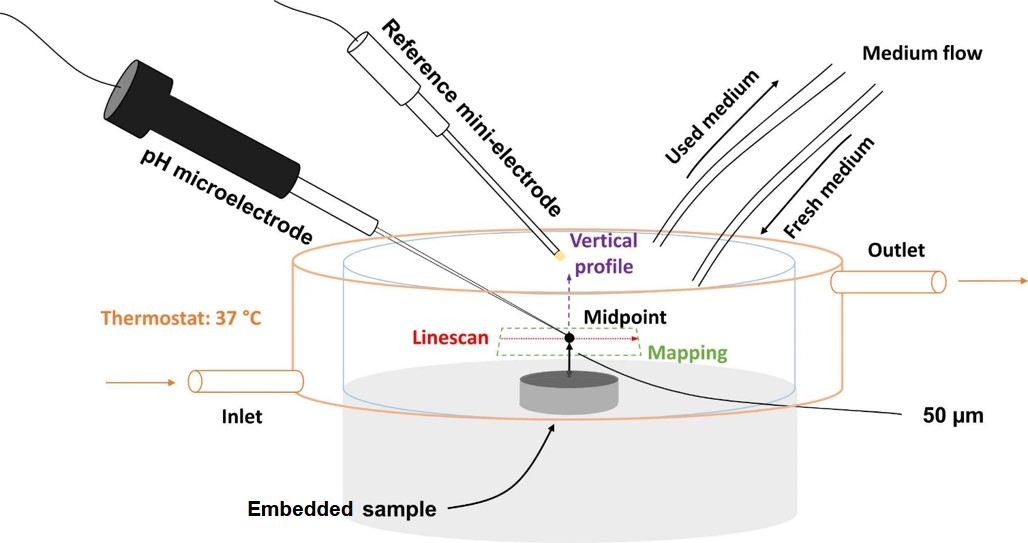
\includegraphics[width=\textwidth]{setup.jpg}
\caption[Fluid flow model construction for comparison with experimental setup]{Fluid flow model construction for comparison with experimental setup} \label{fig:fluid_setup}
\end{figure}

\begin{figure}[h]
\centering
\medskip
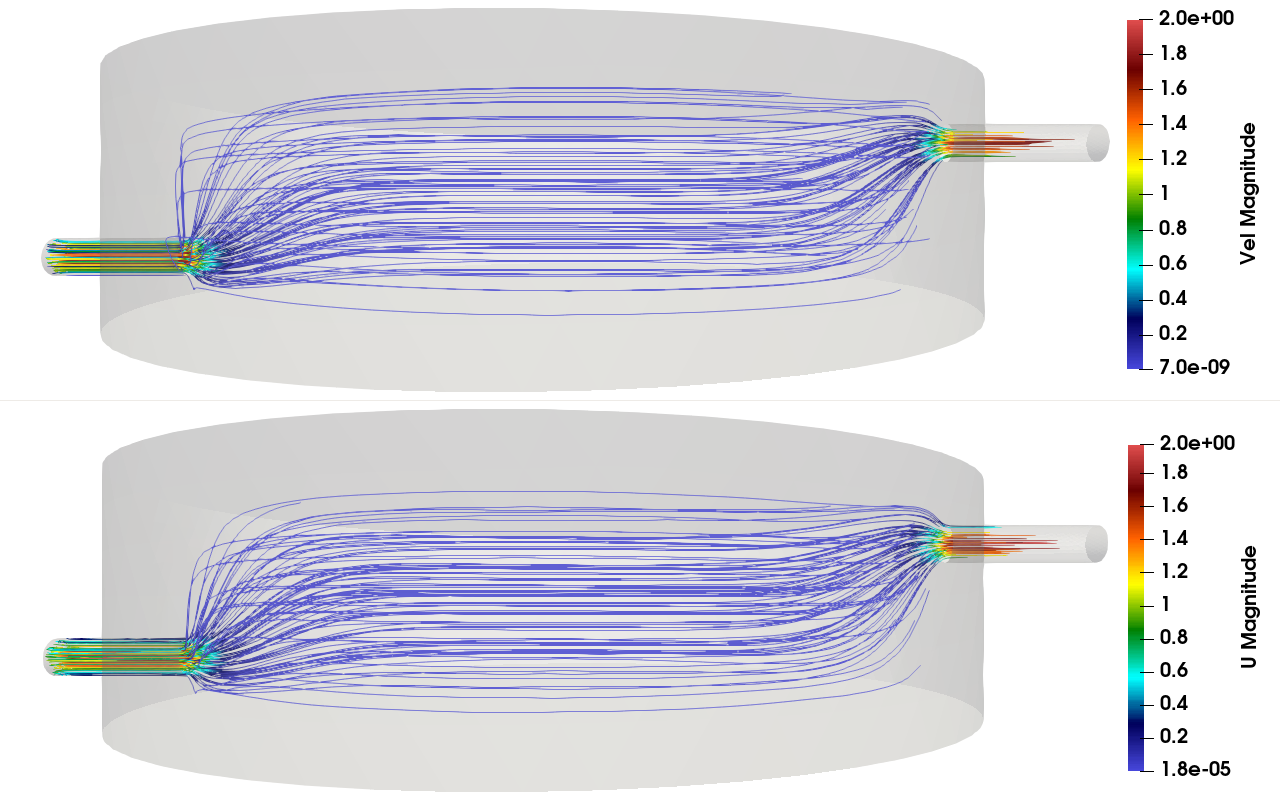
\includegraphics[width=\textwidth]{streamlines_side.png}
\caption[Comparing streamline results of developed CFD code and OpenFOAM - side view]{Comparing streamline results of developed CFD code and OpenFOAM - side view} \label{fig:fluid_streamlines_side}
\end{figure}


\begin{figure}[h]
\centering
\medskip
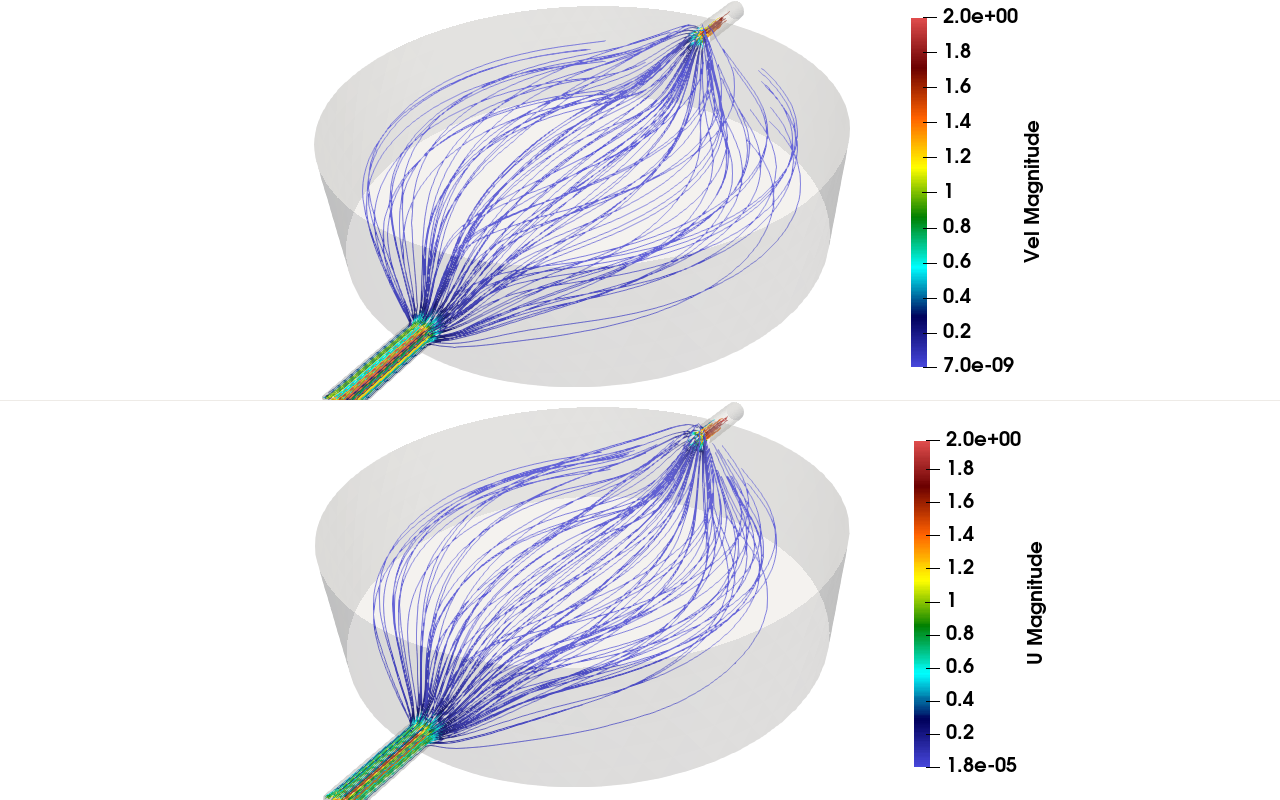
\includegraphics[width=\textwidth]{streamlines_top.png}
\caption[Comparing streamline results of developed CFD code and OpenFOAM - top view]{Comparing streamline results of developed CFD code and OpenFOAM - top view} \label{fig:fluid_streamlines_top}
\end{figure}


\begin{figure}[h]
\centering
\medskip
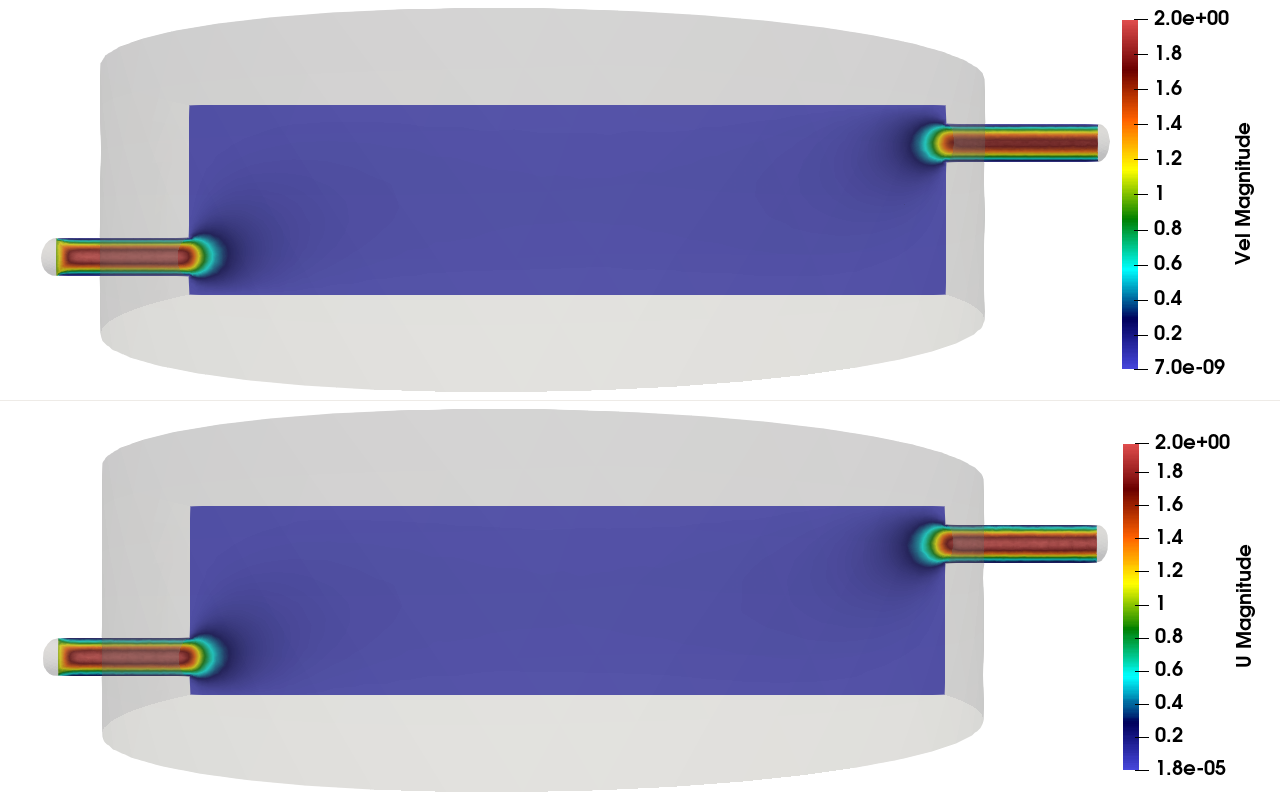
\includegraphics[width=\textwidth]{flow_chamber.png}
\caption[Comparing flow field results of developed CFD code and OpenFOAM]{Comparing streamline results of developed CFD code and OpenFOAM} \label{fig:fluid_flow_chamber}
\end{figure}


\begin{figure}[h]
\centering
\medskip
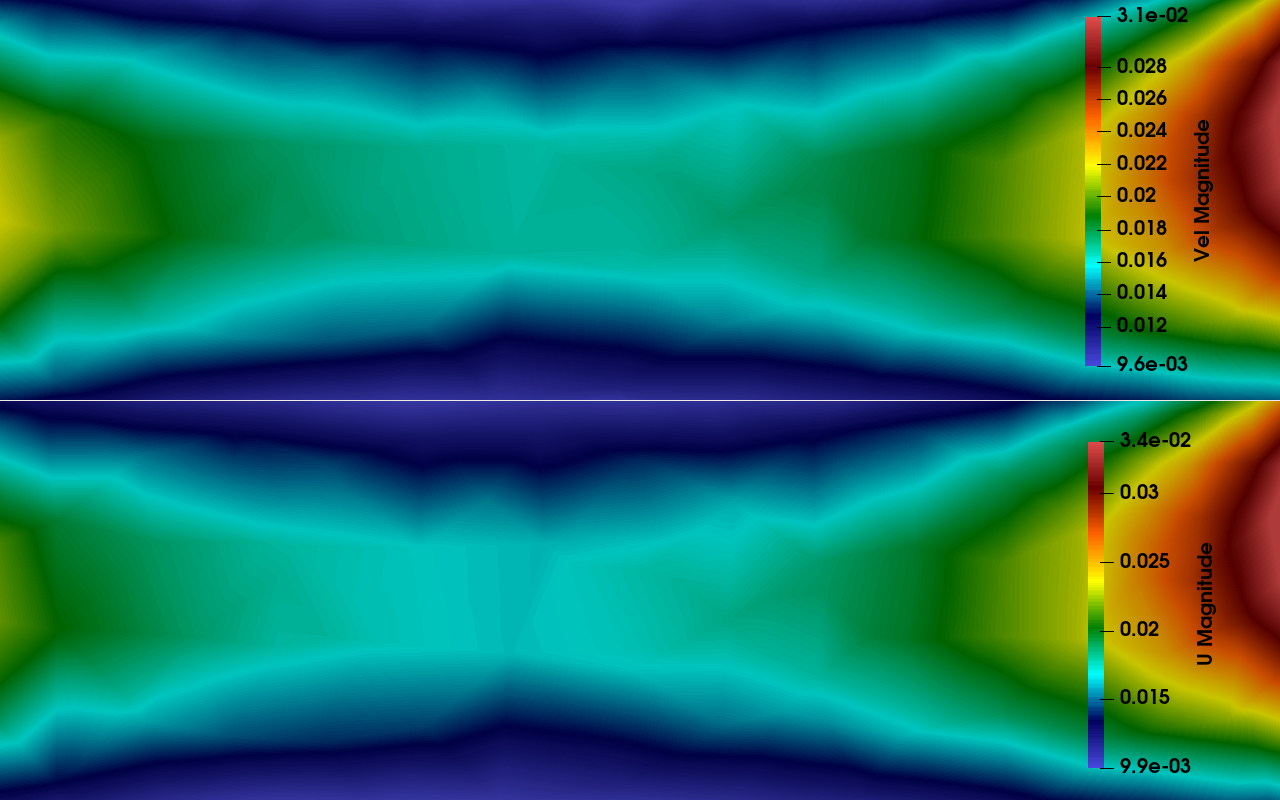
\includegraphics[width=\textwidth]{flow_chamber_zoom.png}
\caption[Comparing flow field results of developed CFD code and OpenFOAM - zoomed view]{Comparing streamline results of developed CFD code and OpenFOAM - zoomed view} \label{fig:fluid_flow_chamber_zoom}
\end{figure}

\begin{figure}[h]
\centering
\medskip
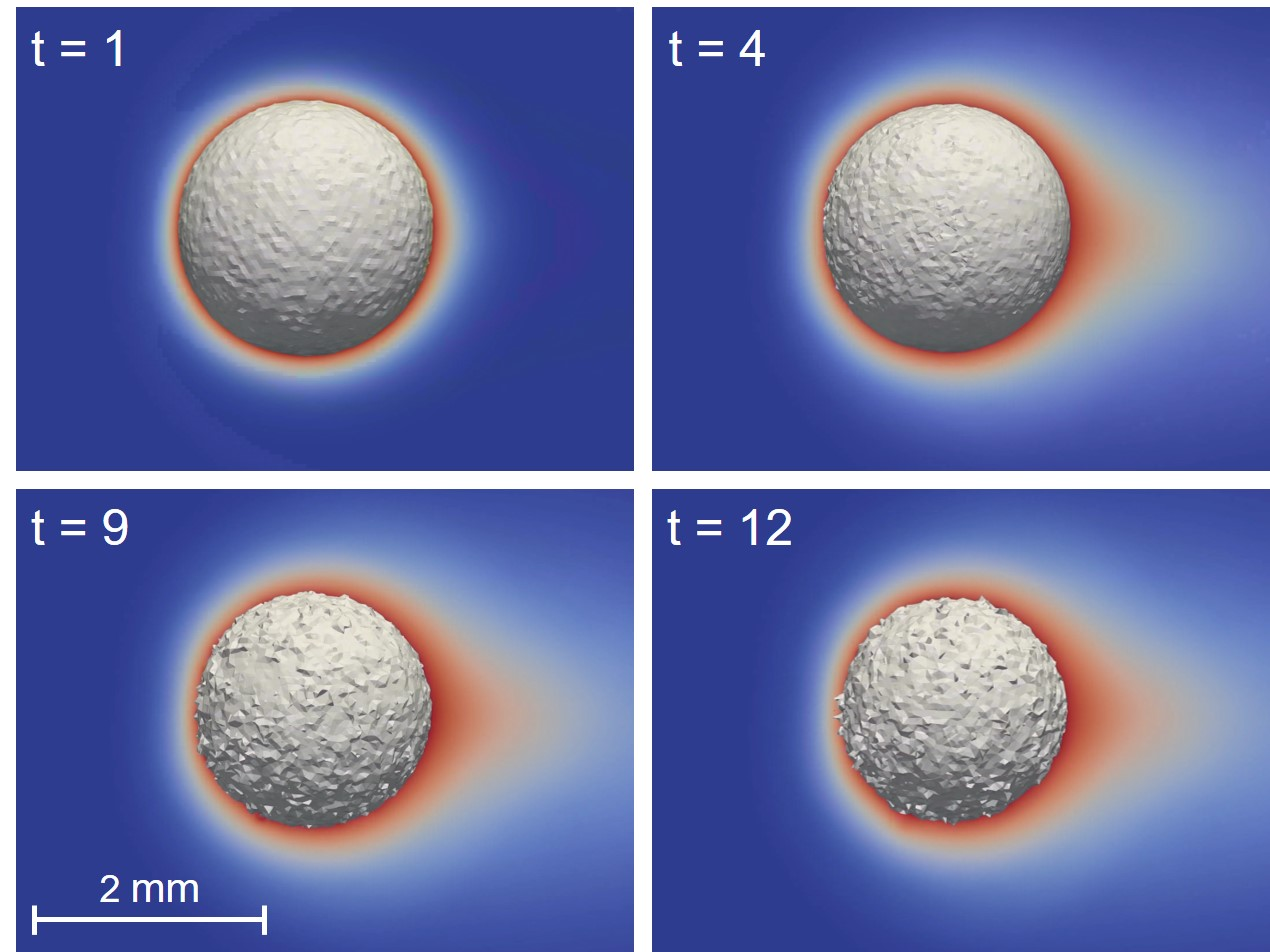
\includegraphics[width=\textwidth]{flow_degrading.jpg}
\caption[Biodegradation simulation results in the presence of fluid flow]{Biodegradation simulation results in the presence of fluid flow} \label{fig:fluid_flow_degrading}
\end{figure}


\begin{figure}[h]
\centering
\medskip
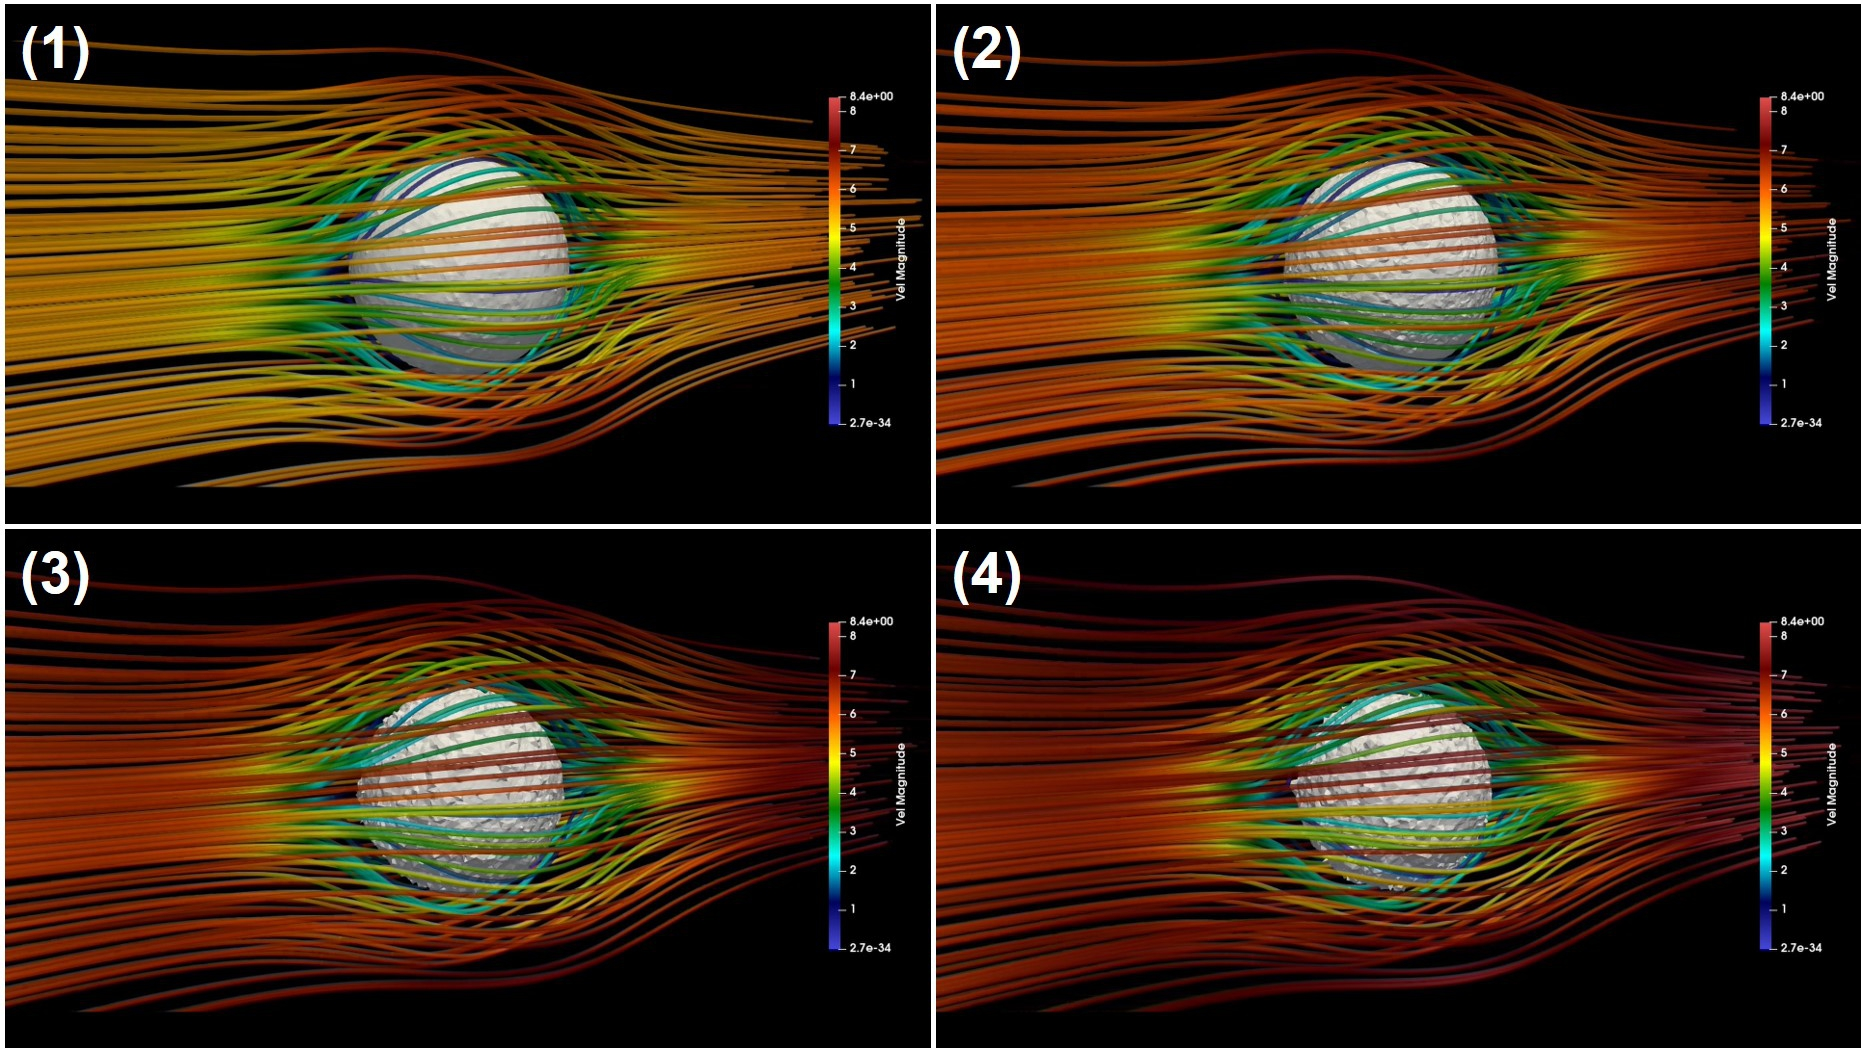
\includegraphics[width=\textwidth]{flow_degrading_streamline.jpg}
\caption[Fluid flow streamlines in the presence of a degrading object]{Fluid flow streamlines in the presence of a degrading object} \label{fig:fluid_flow_degrading_streamline}
\end{figure}
















%%%%%%%%%%%%%%%%%%%%%%%%%%%%%%%%%%%%%%%%%%%%%%%%%%
% Keep the following \cleardoublepage at the end of this file, 
% otherwise \includeonly includes empty pages.
\cleardoublepage

